\documentclass{jarticle}
\usepackage{robomech2022}
\usepackage[dvipdfmx]{graphicx}

\begin{document}
\makeatletter
\title{仮予稿集 条件付き模倣学習とシナリオ}
{―texの練習も添えて-何の種?}
{English Title: Times New Roman, 12pt}
{-English Subtitle: Times New Roman, 10pt-}

\author{
\begin{tabular}{ll}
 \hspace{1zw}正\hspace{1zw}春山健太 (千葉工大)\\
%  \hspace{1zw}学\hspace{1zw}東京 学(西大)& [日本語著者名:明朝体10pt]\\
 % ※協賛・後援団体の会員資格で発表される場合は「正・学」は不要です。
 &\\
 \multicolumn{2}{l}{\small Kenta HARUYAMA, CIT University, hogehohe.jp}\\
%  \multicolumn{2}{l}{\small Jiro SHIBUYA, Robomec Electric Corporation}\\
%  \multicolumn{2}{l}{\small Manabu TOKYO, Nishi University}\\
%  \multicolumn{2}{l}{\small [Authors' names and Affiliations: Times New Roman, 9pt]}
\end{tabular}
}
\makeatother

\abstract{ \small 
Papers submitted must be original, and previously unpublished. The responsibility for the contents of published articles rests solely with the authors and not the society. Copyright of the papers published belongs to the JSME (Japan Society of Mechanical Engineers). [Abstract: Times New Roman, 9pt, 100-150words]
}

\date{} % 日付を出力しない
\keywords{Robot, Manipulation,… (no more than five words) [Times New Roman, 9pt]}

\maketitle
\thispagestyle{empty}
\pagestyle{empty}

\small
\section{緒言}%===========================
% 本文:明朝体・9pt(欧文Times New Roman, 9pt)、文字間隔は1行26文字程度、行間隔は4.2mm程度にして下さい。
本研究では,入出力関係を直接学習するend-to-end学習器により,
経路追従行動を視覚に基づいてオンラインで模倣する手法を提案し,その有効性を実験により検証してきた(以後,岡田らの模倣学習手法と呼ぶ).\cite{okada1}\cite{okada2}
岡田ら模倣学習手法では,測域センサやオドメトリ,などのメトリックな情報を用いて経路を追従する.
この行動をカメラ画像を入力,ヨー方向の角速度の制御信号を目標出力として模倣学習する.
これにより,データセットを自動的に収集しながら学習器の訓練を行い,
学習後はカメラ画像のみで経路を追従することを可能としている.
さらに学習器の入力へ目標とする経路の情報(以後,目標方向と呼ぶ)を加えることで,
行動を条件付けた模倣学習へ拡張を行なってきた(以後,条件付き模倣学習と呼ぶ).
例として,\reffig{fig: path}の場合にはカメラ画像に加え,「左折」という目標方向を入力する.
これにより,学習後のカメラ画像を用いた走行においても,「左折」などの入力により
それに従った経路を選択する機能を獲得している.\cite{haru}.
しかし,前報において,目標方向の生成をカメラ画像を用いた走行においてもメトリックな情報を必要としていた.
\\ 本稿では,シナリオという人間が道案内に用いる情報をロボットのナビゲーション手段と
単眼カメラ画像を用いたロボットの自律移動手法を提案する.
本稿の残りの部分では,関連研究について述べた後,提案する手法のシステムについて述べる.
そのシステムを用いた実験を行い,最後に結言を述べる.
\begin{figure}[h]
  \centering
   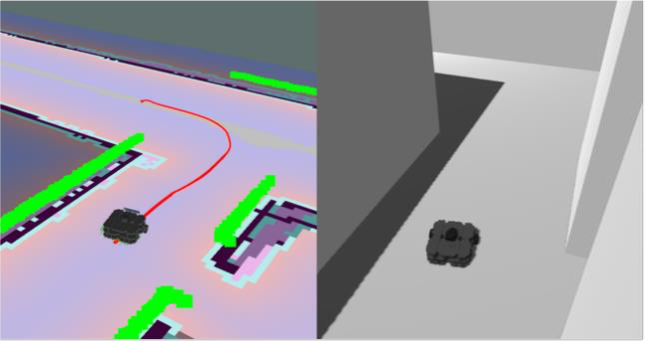
\includegraphics[height=40mm]{./figs/path.png}
   \vspace*{-4mm}
   \caption{Imitation learning of path-tracking}
   \label{fig: path}
 \end{figure}

% \subsection{論文作成に関する注意事項を以下に示します。(中見出し:ゴシック体・9pt・強調文字・左寄せ)}%-----------
% \begin{itemize}
% 	\item 用紙サイズ:A4(210×297mm)とします。
% 	\item 用紙マージン:上下25mm。日本語表題から\textbf{\textit{Key Words}}までの1段組の部分は、左右25mm以上空けて下さい。本文からは2段組とし、左右15mm、段間は6mmとします。
% 	\item 文字のフォント、大きさ:\reftab{tbl: table1}を参照下さい。
% 	\item 図の画質:300dpi以上の画質の高いものにして下さい。
% 	\item 図・表のタイトル:図のタイトルには「Fig.\# English title」、表のタイトルには「Table \# English title」という形式を用い、文中ではそれぞれ「図\#」、「表\#」という表現にして下さい。
% 	\item グラフの軸タイトル:各軸のタイトルに変数記号だけを記述するのは避けて下さい。\reffig{fig: fig1}に示すように、軸を表す語句ならびに単位を記入して下さい。
% 	\item 式:以下に示すように、右寄せで番号をふり、式は中央に配置して下さい。文中では「\refeqn{eqn: eq1}」と表現して下さい。
	
% 	\begin{equation}
% 		M\ddot{r}_{str1} + F_{frk} = Mg
% 		\label{eqn: eq1}
% 	\end{equation}

% 	\item 単位:SI単位系とします。
% 	\item 本文中に文献を引用する場合、引用を表す語句や文の後ろに文献番号(例えば\cite{Shinjuku98})を振って下さい。文献を主語や目的語などに用いる場合、「文献\cite{Shinjuku98}では、・・」などのようにして、番号のみの表現を避けて下さい。
% 	\item 連名の場合には講演発表者氏名の前に○印をつけて下さい。
% 	\item 作成した論文はPDFファイル形式に変換し、PDFファイルのみを学会本部へ提出して下さい。PDFファイルの提出は本講演会ホームページ記載のアップロードのページの指示に従って下さい。
% 	\item[]
% 	\item[※] ただし、PDFファイルの容量は2MB以下、論文のページ数は2頁以上4頁以下とします。なお、印刷原稿の提出は不要ですので、郵送しないで下さい。
% 	\item[※] 講演番号、講演会名、ページ番号は記載しないようにして下さい。
% \end{itemize}
\section{関連研究}
\section{提案手法}
提案する手法を構成する条件付き模倣学習,シナリオ,単眼カメラ画像を用いた通路形状の検出の3つの要素に分けた述べる.
〜では要素を組み合わせた提案手法について述べる.
\subsection{条件付き模倣学習}
条件付き模倣学習で用いるシステムを図〜に示す.
LiDARとオドメトリを入力とする地図をベースとする制御器による自律移動を,学習器を用いて模倣する.
学習器の入力はカメラ画像,目標出力は地図をベースとする制御器の出力するヨー方向の角速度である.
条件付き模倣学習は上記の学習器の入力へ経路の情報である,目標方向を追加している.
また地図をベースとする制御器へ目標方向の生成機能を追加している.
前報ではテスト段階においても,目標方向の生成を地図をベースとする制御器から生成を行っていた.
つまり,テスト時においてもLiDARとメトリックマップなマップを必要としている.
\subsection{シナリオ}
メトリックマップなマップを用いずにロボットをナビゲーションする方法として,
本研究室では〜を提案し,実ロボットを用いた実験により有効性の検証を行なっている.
人の道案内に着目したトポロジカルマップのデータ形式と経路を表現するシナリオの生成法
図〜にトポロジカルマップ及び,その情報を用いたシナリオの生成方法について示す
トポロジカルマップは通路の特徴(ノード)とそのつながりを示すエッジから構成されている.
ノードはID,通路の特徴,エッジの情報を有している.
このトポロジカルマップの情報を用いて,ノード5からノード11へのシナリオを生成すると
三叉路まで直進.右折.突き当りまで直進.停止.」となり,
人の道案内 に似た形式の文章が生成される.
生成したシナリオを用いて自律移動する際には通路の特徴を検出する必要がある.
その際,LiDARを用いる方法,全天球カメラとYOLOを組み合わせる手法を用いている.
通路の検出するタイミングは,通路へ侵入後である.
学習器へ目標方向を指示をするタイミングは,
前述の通り,分岐路に侵入する前に行う必要がある.
そのため,例として,図〜に示した〜めなどの場合には,
2つ目を通過後に「右折」を指示するという手法が考えられる.
しかし,図〜に示したシナリオの場合に,目標とする通路まで〜を指示し続ける方法では,
途中の分岐路において「右折」を選択してしまうことが考えら,通路の特徴を侵入前から事前に把握する必要がある.
そのため,通路の検出手法について,次節で述べる手法を用いる.
\begin{figure}[h]
  \centering
   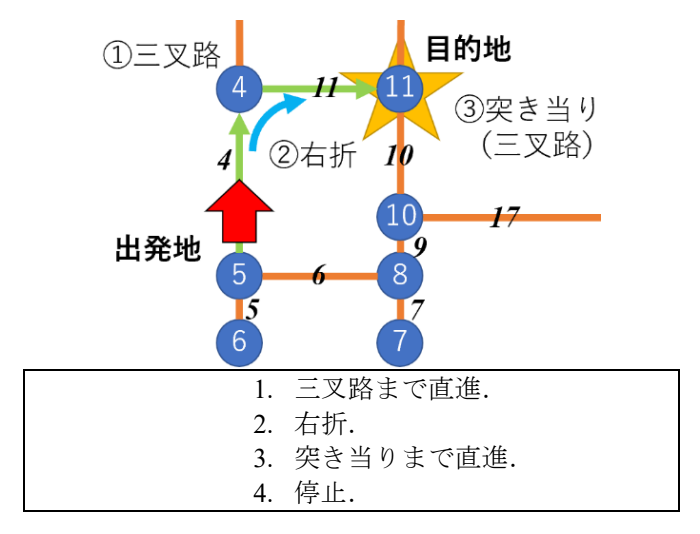
\includegraphics[width=80mm]{./figs/scenario.png}
   \vspace*{-4mm}
   \caption{Example of a scenario}
   \label{fig:scenario}
 \end{figure}

\subsection{単眼カメラ画像を用いた通路形状の検出}
通路の形状を事前に把握する手法として,
セマンティックセグメンテーションを用いて検出手法や,単眼カメラ画像を用いた分類問題
により検出する手法が提案されている.
セグメンテーションを用いる手法では屋外の開かれた環境を対象としているため,
図〜のような屋外環境においては,左右の壁により,
十分に通路を観測することが困難であることが考えらる.
そこで本研究では,〜が行った単眼カメラ画像を用いた分類問題により,
通路検出する手法を参考に実装を行う.
\begin{figure}[h]
  \centering
   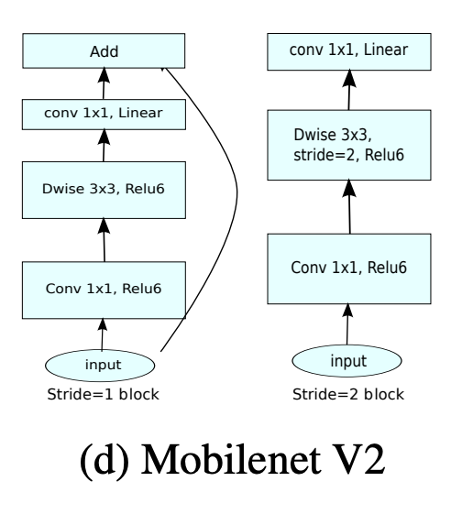
\includegraphics[width=60mm]{./figs/mobilenetv2.png}
   \vspace*{-4mm}
   \caption{Structure of Mobilenetv2}
   \label{fig:mobilenetv2}
 \end{figure}
\subsection{システム}
要素を統合したシステムの全体について,学習器の訓練段階と,訓練後に分けて述べる.
学習器は条件付き模倣学習を学習器,通路の分類を行う学習器の二つを用いる.
条件付き模倣学習に関しては〜で述べた手法で行う.
その際,通路の分類を行う学習器の訓練も同時に行う.分類用のラベルを地図を
ベースとする制御器から行うことで,〜と〜の訓練を同時に行うことが可能である.
訓練後は

\section{実験}
\section{結言}
%※ ただし、PDFファイルの容量は2MB以下、論文のページ数は2頁以上4頁以下とします。なお、印刷原稿の提出は不要ですので、郵送しないで下さい。

%※ 講演番号、講演会名、ページ番号は記載しないようにして下さい。
% ff

% \begin{table}[h]
%  \caption{Type size and typefaces for papers}
%  \label{tbl: table1}
%  \centering
%  \footnotesize
%  \begin{tabular}{|p{7zw}|c|c|c|}
%   \hline 
% 	適用場所	&日本語	&欧文 \\\hline
% 	標準のフォント	&明朝体 9pt	&Times New Roman 9pt \\\hline
% 	日本語表題	&ゴシック体 14pt	&Arial 14pt \\\hline
% 	日本語副表題	&ゴシック体 12pt	&Arial 12pt \\\hline
% 	英語表題	&-&Times New Roman 12pt \\\hline
% 	英語副表題	&-&Times New Roman 10pt \\\hline
% 	日本語著者名	&明朝体 10pt &-\\\hline
% 	英語著者名	&-&Times New Roman 9pt \\\hline
% 	アブストラクト・キーワード	&-&Times New Roman 9pt \\\hline
% 	大見出し	&ゴシック体 10pt	&Arial 10pt \\\hline
% 	中見出し	&ゴシック体 9pt	&Arial 9pt \\\hline
% 	図・表の番号・タイトル	 &-&Times New Roman 9pt \\\hline
% 	文献	&明朝体 8pt	&Times New Roman 8pt \\
%   \hline
%  \end{tabular}
% \end{table}

\begin{figure}[h]
 \centering
  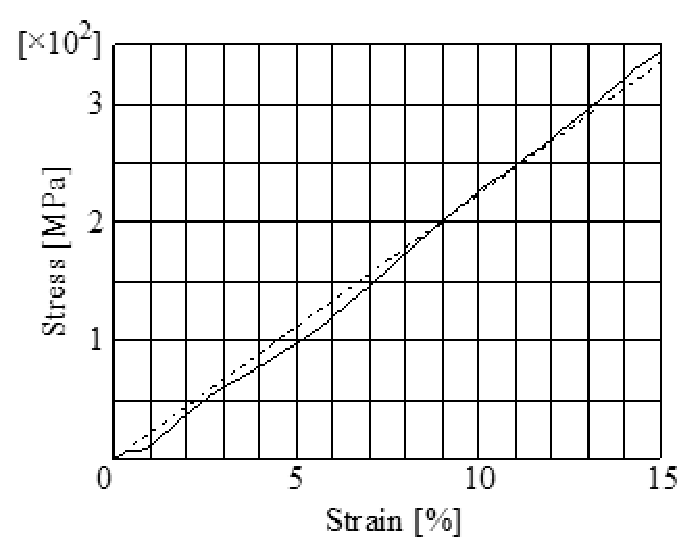
\includegraphics[height=38mm]{./figs/fig1.eps}
  \vspace*{-4mm}
  \caption{Tensile stress-strain diagram}
  \label{fig: fig1}
\end{figure}


\footnotesize
\begin{thebibliography}{99}

\bibitem{okada1}
岡田眞也,清岡優祐,上田隆一,林原靖男“:視覚と行動のend- to-end 学習により経路追従行動 をオンラインで模倣する手法 の提案”,計測自動制御学会 SI 部門講演会 SICE-SI2020 予稿 集,pp.1147–1152(2020)
\bibitem{okada2}
岡田眞也,清岡優祐,春山健太,上田隆一,林原靖男:“視覚と 行動の end-to-end 学習により経路追従行動 をオンラインで 模倣する手法の提案 -経路追従行動の修正のためにデータセッ トを動的に追加する手法の検討”,計測自動制御学会 SI 部門 講演会 SICE-SI2021 予稿集,pp.1066-1070(2021)
\bibitem{haru}
春山健太,藤原柾,清岡優祐,岡田眞也,上田隆一,林原靖男,"視覚と行動のend-to-end学習により経路追従行動をオンラインで模倣する手法の提案 ―経路選択機能の追加―",日本機械学会ロボティクス・メカトロニクス講演会'22予稿集,(2022)
% \bibitem{Shinjuku98}
% 新宿大五朗,渋谷次郎,東京 学,``キャスティングマニピュレーションに関する研究(第1報,可変長の紐状柔軟リンクを有するマニピュレータの提案とそのスイング制御法)'',機論C編, vol.64-626, pp.3854--3861, 1998.

% \bibitem{Shinjuku99}
% Shinjuku, D., Shibuya, J. and Tokyo, M., ``Swing Motion Control of Casting Manipulation,'' IEEE Control Systems, vol.19-4, pp.56--64, 1999.

\end{thebibliography}

\normalsize
\end{document}
